\documentclass[11pt,a4paper,roman]{moderncv}       
\usepackage{graphicx}                 
\usepackage{graphics}
\graphicspath{{Pics/}}  

%\patchcmd{\maketitle}
%  {\hfil}
%  {\hspace*{0.15\textwidth}}
%  {}
%  {}
%\patchcmd{\maketitle}
%  {\setlength{\maketitlewidth}{0.8\textwidth}}
%  {\setlength{\maketitlewidth}{0.67\textwidth}}
%  {}
%  {}
%\patchcmd{\maketitle}
%  {\\[2.5em]}
%  {\hfil\raisebox{-.7cm}{\framebox{\includegraphics[width=\@photowidth]{resum.jpg}}}\\[2.5em]}
%  {}
%  {}

  
% moderncv themes
\moderncvstyle{banking}                             % style options are 'casual' (default), 'classic', 'banking', 'oldstyle' and 'fancy'
\moderncvcolor{grey}                               % color options 'black', 'blue' (default), 'burgundy', 'green', 'grey', 'orange', 'purple' and 'red'

\usepackage{polyglossia}      
\setdefaultlanguage{russian}  
\setotherlanguage{english}    

\setkeys{russian}{babelshorthands=true}
\newfontfamily{\cyrillicfont}{Arial}
\usepackage[utf8]{inputenc} 

\usepackage[scale=0.75]{geometry}



\name{Елизавета}{Голованова}
                              
\address{Лобачевского 88}{119454}{Москва}
\phone[mobile]{+7~(917)~515~3801}                  


\email{golovanovaliza@mail.ru}                               

%Нет, я не нашла фотки получше для резюме))
\photo[90pt][0pt]{resum1.jpg}                       % optional, remove / comment the line if not wanted; '64pt' is the height the picture must be resized to, 0.4pt is the thickness of the frame around it (put it to 0pt for no frame) and 'picture' is the name of the picture file
%\quote{Some quote}                                 % optional, remove / comment the line if not wanted

% bibliography adjustements (only useful if you make citations in your resume, or print a list of publications using BibTeX)
%   to show numerical labels in the bibliography (default is to show no labels)
%\makeatletter\renewcommand*{\bibliographyitemlabel}{\@biblabel{\arabic{enumiv}}}\makeatother
\makeatletter
\@ifpackageloaded{moderncvstylebanking}{%
\let\oldmakecvtitle\makecvtitle
\renewcommand*{\makecvtitle}{%
  {\centering{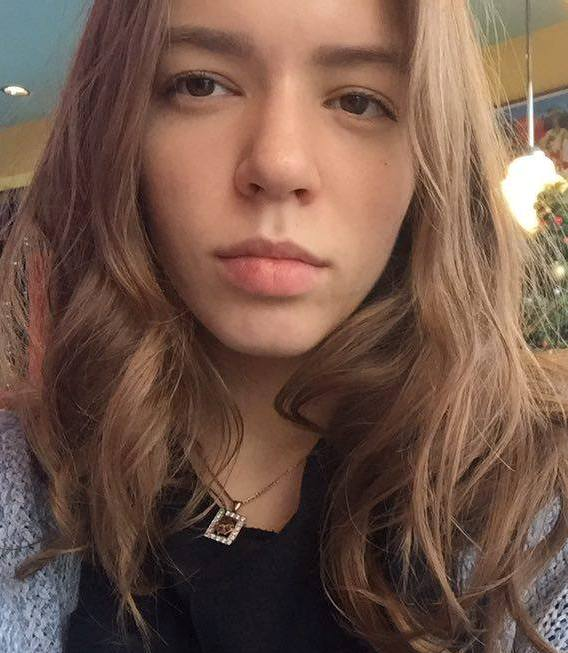
\includegraphics[width=\@photowidth]{resum1.jpg}}\par\vspace{10pt}}%
  \oldmakecvtitle%
}%
}{%
}
\makeatother



\begin{document}
\hspace{1cm}
\makecvtitle

\section{Education}
\cventry{2014--2018}{Бакалавр}{РАНХИГС ПРИ ПРЕЗИДЕНТЕ РФ}{Москва}{}{Экономика}  % arguments 3 to 6 can be left empty
\cventry{2016--2018}{Бакалавр}{Université Grenoble-Alpes}{Гренобль}{}{Экономика}

%\section{Master thesis}
%\cvitem{title}{\emph{Title}}
%\cvitem{supervisors}{Supervisors}
%\cvitem{description}{Short thesis abstract}

\section{Опыт работы}
\subsection{Разное}
\cventry{2015}{Официант}{Farley Girls}{Galveston}{Texas}{Опыт работы за границей в сфере услуг.\newline{}%
Детализация достижений:%
\begin{itemize}%
\item Опыт работы с иностранными клиентами;
\item Опыт работы в иностранном коллективе;
\item Способность быстро выполнять рутинную работу;
\item Способность быстро осваивать новые навыки.
\end{itemize}}

\section{Языки}
\cvitem{Русский}{native}
\cvitemwithcomment{Английский}{upper-intermediate mid-high}{2005-2017}
\cvitemwithcomment{Французский}{pre-intermediate}{2016-2017}
\cvitemwithcomment{Немецкий}{pre-intermediate}{2009-2017}

\section{Компьютерные навыки}
\cvdoubleitem{R-Studio}{Уверенный пользователь}{Excel}{Продвинутый пользователь}
\cvdoubleitem{LaTeX}{Уверенный пользователь}{Wolfram Mathematica}{Базовые знания}

\section{Хобби}
\cvitem{Увлечение 1}{История и быт зарубежных стран}
\cvitem{Увлечение 2}{Классическая и научная литература}
\cvitem{Увлечение 3}{Рисование}

\section{Курсы иностранных языков}
\cvitemwithcomment{MERCY COLLEGE}{Изучение английского языка
в Дублине}{2011}
\cvitemwithcomment{ST. CLARES}{Изучение английского языка
в Оксфорде}{2012}
\cvitemwithcomment{BURLINGTON SCHOOL}{Изучение английского языка
в Лондоне}{2012}

\section{Достижения}
\cvitemwithcomment{ХУДОЖЕСТВЕННАЯ ШКОЛА}{Красный диплом}{2013}

\cvitemwithcomment{КЕЙС-ЧЕМПИОНАТ CHANGELLENGE CUP TECHNICAL}{25\% HQ Award}{2016}

\cvitemwithcomment{КЕЙС-ЧЕМПИОНАТ CHANGELLENGE CUP MOSCOW}{25\% HQ Award}{}


\end{document}

